% csci5271.tex
% this is the main LaTex file
\documentclass{sig-alternate-05-2015}
\usepackage{amsfonts}
\usepackage{graphicx}
\usepackage{hyperref}
\usepackage[hyphenbreaks]{breakurl}

\begin{document}

\title{Link Prefetching: A Defense Against Website Fingerprinting on Tor \titlenote{This report is submitted as a partial fulfillment of {\it CSCI5271: Introduction to Security} course.}}

\numberofauthors{4}
\author{
    \alignauthor
        Vaibhav Sharma\\%
        \email{vaibhav@umn.edu}
    \alignauthor
        Taejoon Byun\\
        \email{taejoon@umn.edu}
\and
    \alignauthor
        Elaheh Ghassabani\\
        \email{ghass013@umn.edu}
    \alignauthor
        Se Eun Oh\\%
        \email{seoh@umn.edu}
\and
    \affaddr{Department of Computer Science and Engineering}  \\
        \affaddr{University of Minnesota}   \\
        \affaddr{Minneapolis, MN 55454}
}

\maketitle
\begin{abstract}
\emph{This paper is written to get an A in the CSCI5271 course.
PERIOD.A++ actually}

\emph{This content will be edited later.} We plan to explore the area of website fingerprinting in anonymization networks starting with the paper Website Fingerprinting in Onion Routing Based Anonymization Networks.
\end{abstract}

% We no longer use \terms command
%\terms{Theory}

\keywords{Website fingerprinting, anonymity, encrypted traffic, Tor}

% section 1
% TJ: let's write it later.
\section{Introduction}
% sections/intro.tex
Anonymizing networks are privacy technologies that provide a mancinism to anonymize internet communications so as to protect users from network eavesdroppers.
Although such systems are able to hide the communication (including both routing information and content), an attacker is still able to obtain different information by analyzing the network traffic.
Network analysis can provide very rich information about message length, timing, and frequency by which an attacker can easily identify the communicating parties, and therefore bypass an anonymizing system.
This problem is known as Website Fingerprinting (WF) attack, where an adversary attempts to recognize the encrypted traffic patterns of specific web pages without using any other information \cite{juarez14, murdoch2005low}.

% we should say, there is lots of work trying to prevent WF attack. And, in this project, we studied most of the state of the art works, and tries to provide a novel defend mechanism [or something similar]

% we want to add a summary about we have done

The remaining sections of this report is organized as follows: Section~\ref{sec2} provides a brief background about Tor anonymity network and website fingerprinting and Section~\ref{sec3} mentions related works on website fingerprinting attacks, defenses and criticisms.
We suggest link prefetching as a defense mechanism in Section~\ref{sec4} followed by experimental evaluation (Section~\ref{sec5})
Section~\ref{sec6} discusses about the feasibility of the proposed defense based on experimental result, and finally conclude our report on Section~\ref{sec7}.



% section 2: (Background)
\section{Website Fingerprinting on Tor}
% \section{Background}
% sections/fingerprinting.tex
% 2. Website Fingerprinting on Tor

This section provides a background on The Onion Router (Tor), the anonymizing systems, and the website fingerprinting attack which can neutralize the anonymity that Tor provides.

\subsection{Tor}

Tor is one of the most popular anonymity networks, which distributes user's communications over several places on the Internet.
The distribution helps user's final destination not to be linked to a single point. Tor can be considered as an overlay network on top of the internet which directs TCP streams to different proxies.
In this network, packets take a random path through several relays, instead of taking a direct route.
These layers cover the user path such that it will not be possible to tell where the data comes from, or where it is going.
Such a pathway in Tor is called a private network pathway.
The Tor client application is responsible of creating this private pathway by incrementally building a circuit of encrypted connections.
The circuit is constructed hop by hop, which means each individual relay is only aware of the previous and next hop.
That is to say, individual relays never can identify the complete path. In order to build circuits, Tor makes use of authenticated DH key exchange encrypted with symmetric keys \cite{TorPage, dingledine2004tor}. Figure~\ref{fig:tor} demonstrates how Tor works.

\begin{figure}[h]
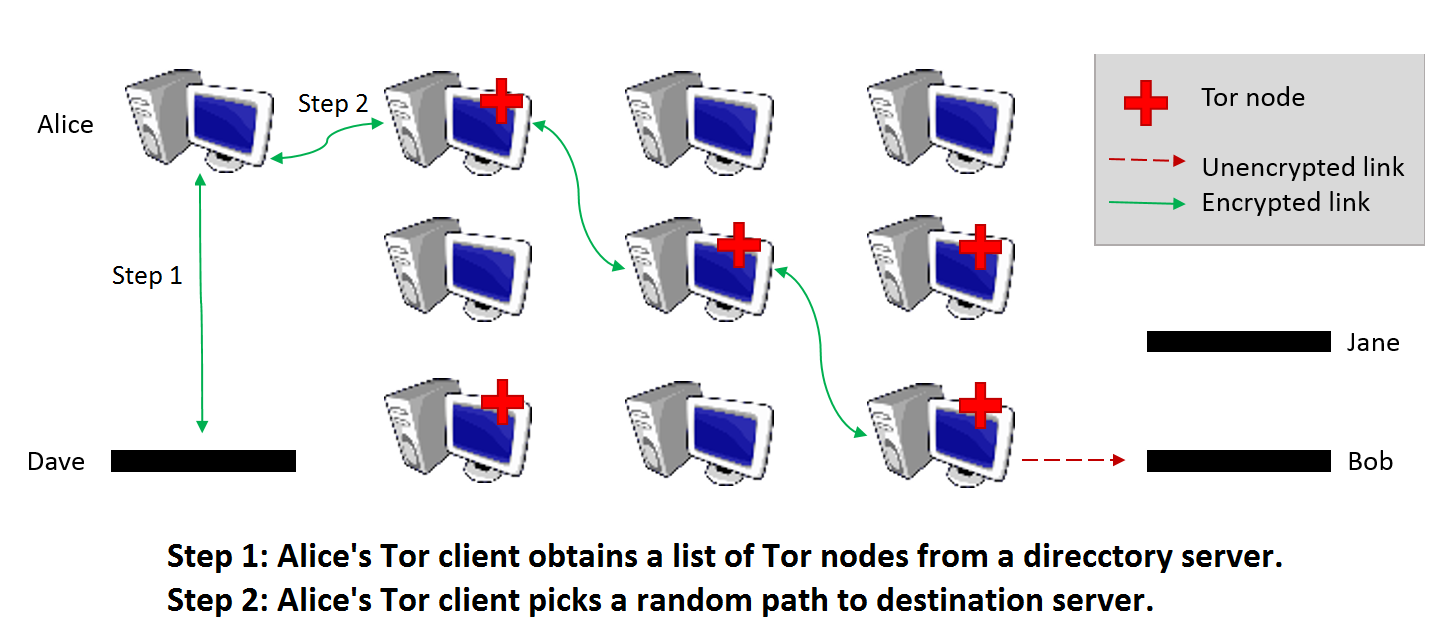
\includegraphics[width=1\columnwidth]{figures/tor.png}
\centering
\caption{The Onion Router (Tor)~\cite{TorPage}}
\label{fig:tor}
\end{figure}

The design described above aims to support a variety of anonymity goals. However, if an attacker can see both ends of the private pathway, Tor will fail.
For example, suppose the attacker watches the Tor relay to which the user enters the network, and also watches the website he visit; in this case, the attacker can correlate volume and timing information on the two sides.
To cope with this problem, Tor came up with the idea of {\it entry guards}, where each Tor client randomly selects a few relays as entry points for her first hop.
If those relays are not observed by an attacker, the user is secure.
But, needless to say, there is always a probability of losing anonymity~\cite{TorPage}.

\subsection{Website Fingerprinting}

Tor does not provide protection against all anonymity problems. In addition, the WF attack is still able to bypass its privacy mechanism. In the case of Tor, WF attack would take place between the user and the Guard node, or at the Guard node itself. In general, attack models can be divided into two categories: "closed world" and "open world" scenarios.  This section describes these attack models.

In the closed world model, the classifier can successfully recognize only web pages that it has already been trained on. Therefore, in this case, we deal with a small set of censored web pages. The open world scenario is when the ability of the adversary can recognize censored pages that might have not seen before \cite{TorBlog}.


Figure~\ref{fig:attack} illustrates the attack model of website fingerprinting. We also consider the WF adversary as local and passive, which means although the adversary is able to eavesdrop on user's traffic, he cannot modify it. It should be pointed out that the adversary will not be able to decrypt the traffic. Otherwise, he would not bother lunching the WF attack. 
MORE EHER!!!!!!!!!!
\begin{figure}[h]

\includegraphics[width=0.7\columnwidth]{figures/attack_model.png}
\centering
\caption{Website Fingerprinting Attack Model~\cite{juarez14}}
\label{fig:attack}
\end{figure}




% section 3
\section{Related Work}
% sections/related.tex
% 3. Related Works

This section surveys attacks/ defenses on/against anonymizing systems, especially Tor. 

\subsection{Fingerprinting Attacks}

The idea of inferring meaningful information based on sniffing and analyzing encrypted SSL packets, which is called deep packet inspection (DPI), was introduced in 1996 \cite{wagner96}.
Later in 2002, Hintz presented the first website fingerprinting attack on an encrypted web proxy.
The attack shows how DPI is powerful enough to identify a specific web site that the user is surfing \cite{hintz2003}.
Since then, a lot of research has been conducted in this area trying either to propose a more realistic WF attack, or a more effective defense mechanism against WF.

Herrmann et al. \cite{herrmann2009} pointed out that widely used anonymous networks such as Tor still failed to defend against WF attack.
They achieved only a 3\% success rate for 775 pages using Multinomial Naive Bayes classifier focusing only on packet sizes.
The WF attacks on Tor suggested by Penchenko et al. \cite{panchenko11} showed more reasonable accuracy with more sophisticated machine learning techniques and diverse features.
Later on, based on \cite{panchenko11}'s attack model, many works such as \cite{wang2013improved, cai2012touching} tried to build more powerful and realistic attacks that improved the accuracy rate up to around 90\% in closed word setting.
They did thorough inverstigation on extracting powerful features such as Tor cells and improving classification method.
Especially, Cai et al. \cite{cai2012touching} had shown that their novel WF attack successfully defeated existing well-known defense mechanisms such as HTTPOS \cite{luo2011}.
However, even though existing works have successfully improved the effectiveness of WF attacks on Tor, underlying assumptions for experiments significantly simplified real world setting.
As Juarez et al. \cite{juarez14} pointed out that existing WF attacks are unrealistic with assumptions such as the client setting, we decided to focus on building more robust and practical defense mechanisim instead of developing advanced attack models to improve the accuracy rate.
%%%TODO \textbf{please add  or modify the comparison of our work to existing works}

%Generally speaking, attacks on anonymizing networks take a variety of approaches; some of the attacks tries to discover the identity of the anonymous user, others focus on uncovering the private pathway, and others attempt to identify the servers users interact with  \cite{cai2012touching}.


\subsection{Defense Mechanisms}

Defense mechanisms are usually developed at the IP/TCP level by changing the pattern of traffic.
For example, they splited packets into multiple packets, injected spurious packets into the traffic, or involved  padding packets to prevent from leaking features of traffic.
A study performed in \cite{fu2003} suggested to transmit packets at random intervals as a defense mechanism against traffic analysis.
Another defense technique proposed in \cite{wright2009}, called traffic morphing, uses some tricks to change a traffic pattern to disguise new or existing other traffic.
However, since their approach still leaks the information such as packet order, attacks that work without packet size information can easily defeat their mechanism.

In \cite{luo2011}, Luo et al. proposed novel HTTP/TCP level defense mechanisms against some analysis attacks by changing window sizes and the order of packets in the TCP stream.
Besides, at the HTTP level, they tried to inject some extra data into HTTP GET headers, generate some irrelevant HTTP request, and re-order requests.
The Tor community also introduced "randomized pipelining" \cite{perry11} to defend the WF, by having the browser load the web content in a random order.
Despite such techniques, the proposed attack in \cite{cai2012touching} managed to successfully recognize target web pages with the accuracy of 87\%. 
Howerver, all exisitng defenses have not been neither efficient nor effective for fancy WF attacks. %This attack is able to ignore packet sizes, while most of the attacks on Tor work based on packet sizes.
In contrast, our work more focuses on utilizing existing HTML systax that is link prefetching shown in Section 4, which subsequently does not accomodate extra cost.

\subsection{Criticism}

In the literature, some work always debate over the practical feasibility of the WF attack. This section tries to summarize issues questioning the practicality of WF.

There are many different factors that play a role in the success of WF.
The main criticism is that academic papers usually oversimplify WF attack models by making some unrealistic assumptions over users' browsing habits, training and testing traces, even the version of Tor used for testing/ training.
In \cite{juarez14}, it is discussed that the studies performed in \cite{cai2012touching, herrmann2009, panchenko11, wang2013improved, shi2009} simplify the problem and overestimate the adversary's capabilities.

Another criticism is that all works lunch attacks on individual pages, instead of overall websites.
So, although the attack is called website fingerprinting, it is actually about webpage fingerprinting.
In addition, there are some main factors, including the the hypothesis state space and the size of the instance space, that affect the accuracy of a classifier.
Even, the number of training samples provided to the classifier and false positive rates matters.
Since reliable feature information is constant, with the increase in the number of classification categories, the classifier eventually runs out of descriptive feature information, which causes either true positive accuracy goes down or the false positive rate goes up.
A Tor blog article~\cite{TorBlog} discusses that the effects of such factors are quite observable in the papers with a sufficient world size.

Although more attention should be paid to the scenarios by which attacks are evaluated, we should not dismiss WF as a threat. However, \cite{TorBlog} argues that, due to theoretical and practical issues, realistic WF attacks are hard to lunch on Tor. Therefore, it claims that even simple defenses could protect Tor users against WF. It seems that the Tor community believes that defense mechanisms do not need to be very complicated to be effective.

To the best of our knowledge, none of the defense techniques has investigated the effect of link pre-fecting on WF. In the next section, we will describe the concept of link pre-fetching. Since most of the defenses are applied at the Tor network, they are required to be acceptable by the Tor community. However, we aim to propose a defense technique which can also be used by the website owners. 
\subsection{Web Prefetching}
Web prefetching has been widely used to reduce the latency for users. Fan et al.\cite{Fan1999} introduced the first prefetching between caching proxies and clients. Chen et al. \cite{Chen2003} pre-fetched web pages that will be visited near future. In addition, there have been several works using prefetching over anonymous network. Nguyen et al. \cite{} prefetched web components of web page, which users are visiting, to solve the delay performance of Tor. They set two proxies, one sits between the client and browser, and the other sits between the exit relay and the website. Even though they successfully improved tor performance, the extra setting of proxies and the communication over them are not good in terms of security since we need to trust them. (e.g., proxies are compromised by adversaries). In contrast, we do not enforce any additional setting on tor network as well as client-side to hinder from such additional security risks.  \textbf{please add  or modify the comparison of our work to existing works}




% section 4
\section{Link Prefetching as a Defense}
% sections/prefetching.tex
% TJ WILL WRITE THIS SECTION !!!

%This section explains the concept of link prefetching and discusses a possible usage of it as a defense mechanism against fingerprinting attacks on Tor.
A classifier used in a website fingerprinting attack can distinguish the differnce between two classes of packets when the difference is consisntent between them~\cite{Cai:2014kjb}. % "A systematic approach to ...", 2014
Thus, intuitively, a classifier would work the best if the difference in the same class is minimal and the difference among heterogeneous classes is high at the same time.
However, when variance among fingerprints in the same class is high, a classifier would not be able to characterize it clearly or at least the detection rate using the classifier would be low.
This is the basic idea of using prefetching as a defense mechanism; our conjecture is that we can use prefetching to manipulate the number and size of incoming and outgoing packets in order to increase the variance among packets in the same class.

This section explains the concept of link prefetching, discusses its effect on website fingerprints and argue its possible usage as a defense mechanism.

\subsection{Link Prefetching}

% introduction about link prefetching
Link prefetching is a HTML syntax that gives the web browser hints about which page the user is most likely to visit in a near future~\cite{fisher2003, fisher2004link}. 
The pages and resources to pre-fetch are specified in the web page so that the web browser can silently load them (or pre-fetch them) after an idle time.
Since the pre-fetch happens only after the page is fully loaded, it does not sacrifice the loading time of the requested web page.
Moreover, it can save the loading time for the pre-fetched pages and thus improve the user experience by caching the {\it future} contents.
It was first suggested by Mozilla Foundation in 2003 and supported by most modern browsers nowadays.

\iffalse %commented out
Once the web contents provider is reasonably certain about which links the users are most likely to visit next, it can improve the user experience by saving the loading time. 
Particularly, it is most effective if the content provider may be reasonably certain which links users are going to visit next.
Having been first suggested by Mozilla Foundation, it is adopted by most modern browsers nowadays.
Today's web browsers makes use of a specific syntax called \emph{pre-fetching}, which was proposed as a draft standard by Mozilla.
Using pre-fetching, browser can predicts documents likely to be visited by the user in the near future.
Therefore, based on the hint provided by pre-fetching a browser is able to fetch those documents a head of time.
In fact, it is the web page that provides a set of pre-fetching hints for the browser.
Then, loading the page and passing an idle time, the browser starts to pre-fetch and cache specified documents.
Needless to say, this mechanism improves efficiency.
\fi
% Insert a figure of "prefetch-network" which shows the network traffic.
% explain about how prefetching actually works 

The resources to prefetch can be simply specified in {\it HTML} using a {\tt link} tag~\cite{nottingham2010}.
For example, a {\tt link} tag {\tt <link rel="p\-refetch" href="/page2.html">} tells the browser to pre-fetch a {\it html} file named {\it page2.html}.
Resources other than a {\it HTML} web page can also be pre-fetched similarly using the same syntax.
There are also some variations for different types of prefetching -- DNS prefetching, which is specified as {\tt <link rel="dns-prefetch" ..>}, is supported by {\it Mozilla Firefox} and {\it Google Chrome}, and {\tt <link rel="prerender" ..>} also does the same job as {\tt prefetch} in {\it Google Chrome} and {\it Microsoft Internet Explorer}.

Figure~\ref{fig:network} illustrates how prefetching actually works in a browser ({\it Google Chrome}).
This page is set up arbitrarily by the authors to demonstrate link prefetching, and contains a link pre-fetch tag that specifies a big image (the image on the left side labeled as {\it prefetch}).
When the prefetching is off, this image shall be requested only when a user puts his mouse cursor on it (mouse over).
However, it can be seen on the network timeline (right bottom) that the image is pre-fetched right after loading the page.
This is indicated by a long blue bar on the second row for the file named ``{\it Very-high...}'', and it is long because the size of the file is relatively big ({\it 3.5 MB}) that it took a longer time to download.
Please also note that the time it took for loading the image when the user actually requested (by putting his mouse on it) was very short, because the image had already been pre-fetched that the browser merely loaded it from the cache (as shown in the {\it size} column on the fourth row).

\begin{figure*}[t]
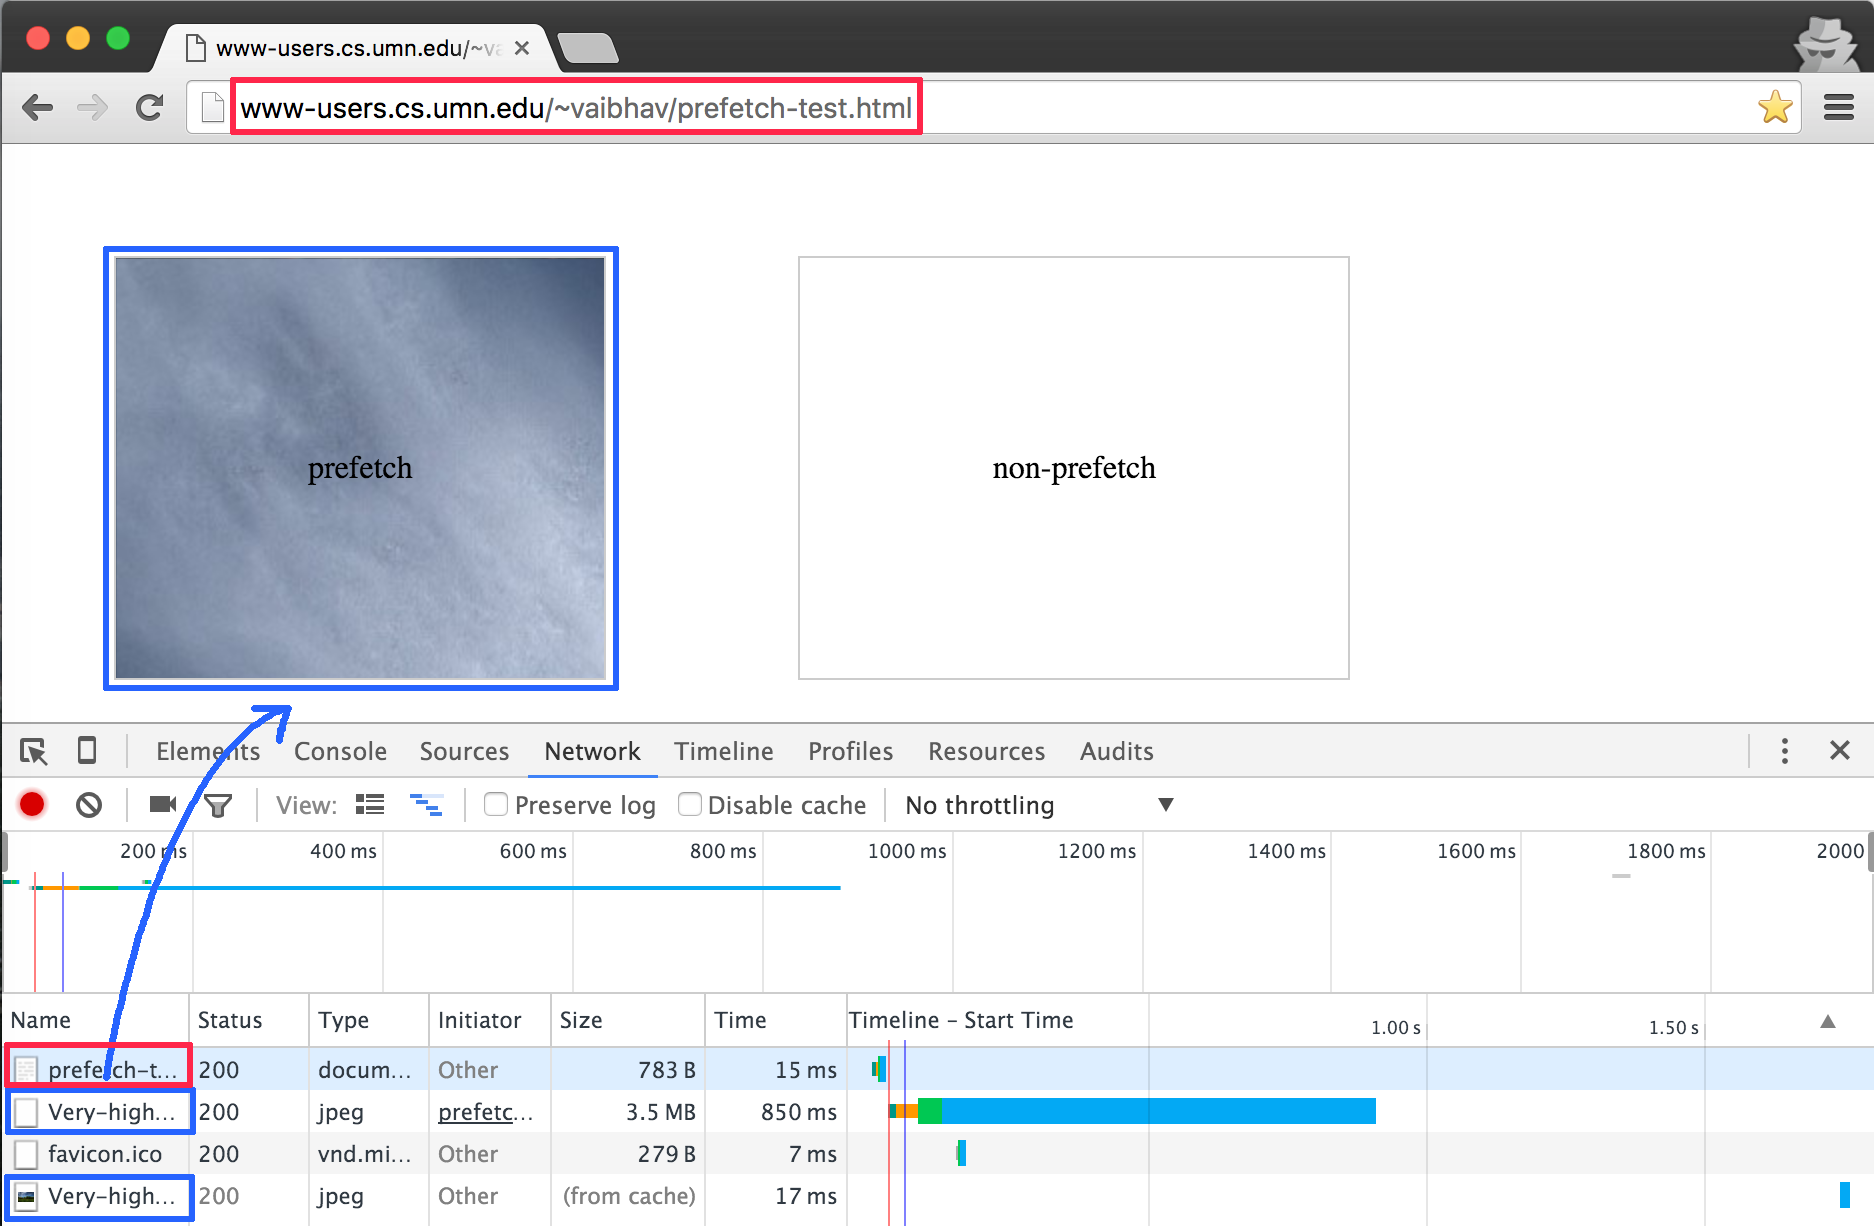
\includegraphics[width=\textwidth]{figures/prefetch-network-edited.png}
\centering
\caption{Network timeline showing pre-fetch}
\label{fig:network}
\end{figure*}


\subsection{The Effect of Prefetching on Website Fingerprint}
% cite some papers to describe about the features that are used for attacks,
% and explain why prefetching change the feature.
% Vaibhav says: put the intuition down 

% TODO: write few sentences as an intro
% We explained through an example how prefetching can affect the

% defenition of a fingerprint

%TODO: rewrite
\iffalse
Link prefetching obviously affects the traffic by sending additional request for prefetching items, and by prefetching those items after an idle time.
However, to what degree it affects the website fingerprint has not been studiedto the best of our knowledge.
This subsection first illustrates how the prefetching affects the number of packets being transferred as an example, and then discusses what features of fingerprint prefetching can possibly affect.
\fi


\subsubsection{An Example of prefetching packet sequence}

\begin{figure}[h]
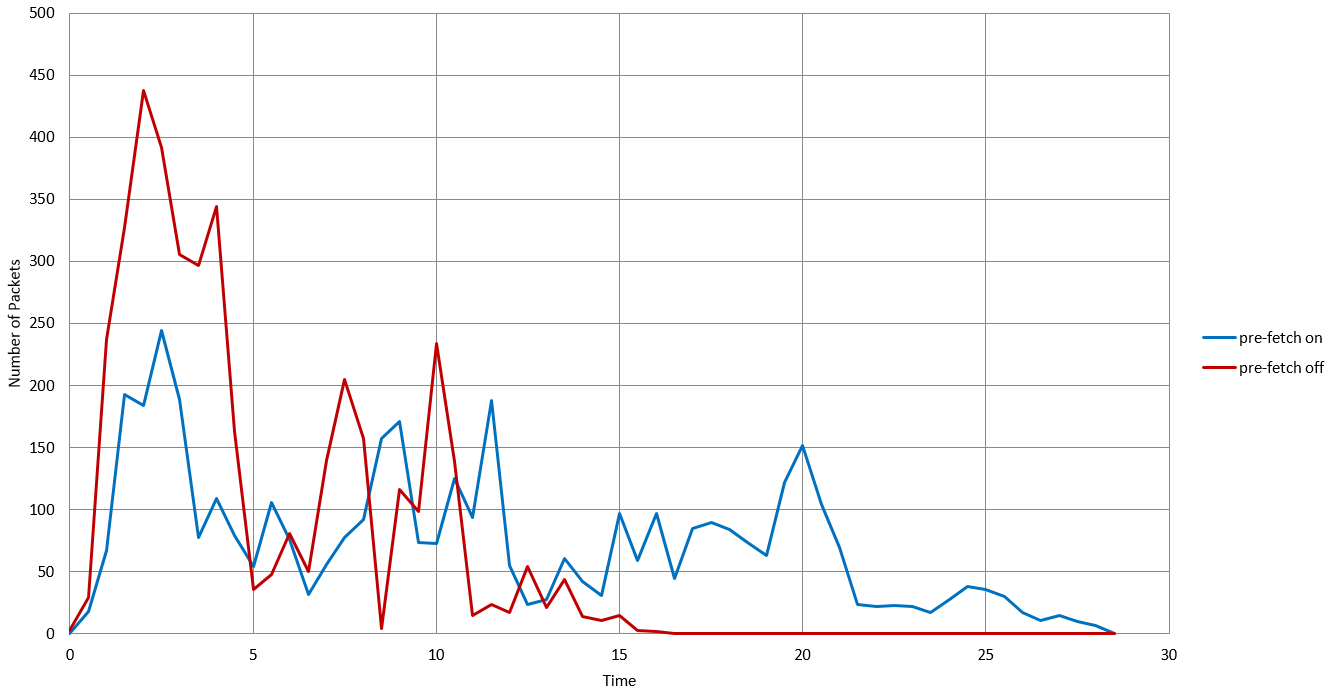
\includegraphics[width=0.95\columnwidth]{figures/prefetch.png}
\centering
\caption{A website fingerprint for pre-fetch on/off cases}
\label{fig:prefetch}
\end{figure}

%The idea of studying the effect of prefetching on Tor network is not new~\cite{something}.
Figure~\ref{fig:prefetch} illustrates a website fingerprint in terms of inter-packet timing, where the {\it x-axis} represents time in seconds and the {\it y-axis} represents the number of packets captured during a certain time interval ({\it 500 ms}).
The solid line depicts the packets captured while prefetching was enabled, and the dashed line depicts when the pre-fetch was disabled in the browser settings.
Both the cases are captured for the same web page, which is the first page of {\tt wired.com}.
However, the number of packets are slightly different for each case (4055 for the {\it off} case while 4218 for the {\it on} case), because the prefetch-on case obviously requests more resources for caching purpose. 
The elapsed time for loading the whole page was also different, but this variance is mainly due to the difference in network condition because all the packets are more scattered throughout time compared to the pre-fetch-off case.
When we ignore the speed difference, we can see that the four peaks of the two lines are roughly the same that if we capture the packets multiple times for the same website, we can characterize how the {\it fingerprint} of a specific website looks like.
Please note also that inter-packet timing is only one of many features for characterizing website fingerprint.


\subsection{Fingerprint Features}

Since all the traffic on Tor is encrypted, fingerprinting attacks blindly analyze a sequence of packets without knowing its contents, and extract {\it features} which characterizes a fingerprint.
The attacker then trains his/her classifier on multiple packet sequences from the set of website, for a set of features that attacker determined to use.
In this subsection, we summarize the definition of the four most popular features defined by Cai et. al.~\cite{Cai:2014kjb} to discuss the effect of prefetching on this features in the following subsection.

{\bf Packet Sequence}:
A packet sequence $P$ can be written as $P = \langle(t_1, l_1), (t_2, l_2), ..., (t_n, l_n)\rangle$ ~\cite{Cai:2014kjb}, where $t_i$ is the time relative to $t_0$ which is 0, and $l_i$ is the byte length of the $i$-th packet.

{\bf Unique Packet Lengths}: 
Most packets 
\begin{equation}
(\exists L \in P_l | L \notin P'_l ) \vee (\exists L \in P'_l | L \notin P_l)
\end{equation}

{\bf Packet Length Frequency}:
When $n_L(P_l)$ is the number of times packet length $L$ appears in $P_l$,
\begin{equation}
\exists L|n_L(P_l) \neq n_L(P'_l) \wedge n_L(P_l)>0 \wedge n_L(P'_l) >0
\end{equation}
In other words, $P$ and $P'$ have different packet length frequencies iff there exists a packet with length $L$ that appears different times in the two sequences.

{\bf Packet Ordering}:
When $M_l$ is the multiset of packet lengths in $P_l$ without ordering, two packet sequences $P$ and $P'$ have different packet ordering iff:
\begin{equation}
M_{ l }=M'_{ l }\wedge P_{ l }\neq P'_{ l }
\end{equation}

{\bf Interpacket Timing}:
\begin{equation}
\exists i, 1 \le i \le \mathit{min}(|P|, |P'|) : (P_t)_i \neq (P'_t)_i
\end{equation}


\subsubsection{The Effect of Prefetching on the Features}

Existing fingerprinting attacks extract {\it features} from a sequence of packets to characterize a distinct characteristic of a website.
The most popular features that have been used in the previous works for classification are unique packet lengths, packet length frequency, packet ordering, and interpacket timing.
Existing works on website fingerprinting considers a sequence
Packet lengths
Packet length frequency
Packet ordering.
Interpacket timing

Packet sequence.


% section 5
\section{Experimental Evaluation}
% sections/experiment.tex

\section{Research Question}

\section{Effects of Pre-Fetching on Fingerprinting}
In this section, we will write  about our experiments. We are planning to conduct two sets of experiments. If we consider the network traffic, the number of packages go upstream depends on the number of pre-fetching requests, and the number of downstream packages coming depends on the size of resources that should be pre-fetched. Therefore, it is obvious that pre-fetching would affect the fingerprint of the traffic of a particular website.  \emph{should be completed.}

\subsection{Investigate Pre-Fetching Effects on top 60 Popular Websites}
We are running experiments to see how pre-fetching affects the websites' fingerprints.
After doing some search on top popular websites, we put together a small crawler by which we learnt that only around 60 of all 6000 websites are use pre-fetching mechanism. We are capturing traffic of these websites in two different modes: 1) with enabled pre-fetching, and 2) with disabled pre-fetching. We are working on feature extraction, and about to decide which classifiers to use for the learning phase.
Ultimately, we plan to conduct two sets of experiments. One sort of experiment is to compare two series of the captured packets and find the accuracy number with the help of a classifier, by which our goal is to provide an evidence to see if pre-fetching really affects fingerprints of websites. So, if the result will be positive, we will perform another set of experiment, which kind of simulates a sub set of those 60 websites. Then, we will see how (altering) the size of pre-fetching affects fingerprinting attacks/ defense mechanisms.


\subsection{Effect of Pre-Fetching Packets Size on Fingerprinting Attacks}
Here, we will explain our second experiment. We will simulate a sub set of webpages we investigated in the previous experiment. Then, we will equip them with a mechanism so that they can affect the downstream traffic and finally their fingerprint. Then, we will analyze the result to see how this idea contributes to the effectiveness of attacks and defense techniques.


Research Questions
\begin{enumerate}
\item
{\bf RQ1}: Does prefetching itself provide an extra degree of defense?
\item
{\bf RQ2}: Can prefetching be used as a browser-side defense mechanism?
\end{enumerate}

\begin{table}[]
\centering
\caption{Experiment design to answer {\it RQ1}}
\label{table:prefetch}
\begin{tabular}{lllll}
\cline{1-3}
\multicolumn{1}{|l|}{victim \textbackslash attacker} & \multicolumn{1}{l|}{prefetch on} & \multicolumn{1}{l|}{prefetch off} &  &  \\ \cline{1-3}
\multicolumn{1}{|l|}{prefetch on}                    & \multicolumn{1}{l|}{(1)}         & \multicolumn{1}{l|}{(2)}          &  &  \\ \cline{1-3}
\multicolumn{1}{|l|}{prefetch off}                   & \multicolumn{1}{l|}{(3)}         & \multicolumn{1}{l|}{(4)}          &  &  \\ \cline{1-3}
                                                     &                                  &                                   &  & 
\end{tabular}                  
\end{table}

\begin{enumerate}
\item
We speculate that prefetching itself might provide extra defense because of the extra packets.
It can also be the case however, prefetching websites are more vulnerable to fingerprinting because of the extra prefetch packets that shows distinct prefix.
\item
This case is unlikely since prefetching is on by default. We assume that victims will more likely be using Tor under the default setting.
\item
This case is what we are most curious about, whether a victim can confuse an attacker by simply turning prefetching setting off of his browser.
\item
This case simulates a situation where a victim is loading any other websites that does not prefetch any resource.
This can be used as a comparison case.
\end{enumerate}


% section 6
\section{Discussion}
% sections/discussion.tex
The performance of link prefetching as a defense mechanism depends on the values used by the webpage for the number of prefetching requests made and the total size of prefetched responses. 
A large number of outgoing requests and incoming responses would make the network prefetching traffic indistinguishable from the normal traffic required to display the webpage.
If a webpage \textit{A} is to make its own network traffic fingerprint similar to another webpage  \textit{B}'s network traffic fingerprint, assuming that webpage \textit{A} currently has a smaller fingerprint than webpage \textit{B}, it should create prefetching network traffic to compensate for the difference in the network traffic fingerprints of \textit{A} and \textit{B}. 
This can further be generalized to the open world model where every webpage can trigger a set of prefetching requests and responses which change its fingerprint to be more similar to a different webpage which has a larger fingerprint. 
This can work for fingerprints which use coarse-grained features as well as fine-grained features.
e.g. a webpage \textit{A} that finds another webpage \textit{B} that creates \textit{K} more outgoing packets resulting in an increase in the total incoming packet size of \textit{S} can simply issue \textit{K} prefetching requests for resources that have a total size of \textit{S}. 
It should however be noted that webpage \textit{A} would have to make requests for resources that are unlikely to be currently cached by the browser.\\
Some attacks may also choose to look at only the first 50 or 100 packets that show up in a packet capture for a given webpage and try to develop a fingerprint using only those packets. 
While the question of the number of packets to be used to create a fingerprinting is definitely interesting, it also needs to be further investigated how many prefetching request and response packets appear in such packet captures. 


% section 7
\section{Conclusions}
% sections/conclusion.tex

%What we have done in this work is so cool and awesome.
%What you may criticize will all be put here as ''future work''.

%This section will conclude the result of our experiments. Finally we will provide some evidence to show how pre-fetching affect fingerprinting attacks. Based on our result, we are planing to suggest some defense mechanisms.
We proposed a new method for defending against website fingerprinting attacks on the Tor anonymity network. 
Link prefetching allows web pages to specify resources which are expected to be downloaded by the browser in the near future and provides web developers with an opportunity to improve user experience on their websites. 
We presented how link prefetching can be useful not only for improved browsing experience but also for acting as a defense mechanism against fingerprinting attacks. 
We showed the effect of link prefetching on different features used by fingerprinting attack classifiers. 
We formulated the challenge of using link prefetching as a defense mechanism in the form of two research questions and designed experiments to evaluate answers to our research questions. 
We create three different classifiers to evaluate the effect of the link prefetching setting on existing real world link prefetching performed by 60 of the 6000 most popular Alexa websites and found the existence of prefetching traffic to reduce the accuracy of classifiers.
We then tried to evaluate the effect of changing the parameter values on the fingerprintability of a webpage but found that the Tor browser does not honor the prefetching requests specified in our test webpage. This behavior deviates from the expected behavior of downloading the prefetching requests once the webpage itself has finished downloading. Finally we discussed how a webpage can calculate the value of the number of prefetching requests and size of prefetched responses in order to disguise its fingerprint. 



\section{Acknowledgments}
<<<<<<< HEAD
This is a research project for CSCI5271, University of Minnesota.
%The authors appreciate Professor Stephen McCamant for telling geeky jokes in classes all the time.
The authors acknowledge the guidance of Professor Stephen McCamant
throughout the course of this research project.
%This is a research project for CSCI5271, University of Minnesota.

\bibliographystyle{abbrv}
\bibliography{csci5271}

\end{document}
